\chapter{Bio-informatique et analyse des séquences}\label{ch:b3:bioinformatics}

Un biologiste qui vient de séquencer un gène d'un ver des grands fonds
colle ses \num{300} acides aminés dans un formulaire en ligne et
apprend, trois secondes plus tard, que la protéine est une cousine
lointaine d'une kinase humaine, avec \qty{31}{\%} d'identité sur
\num{280} résidus et une probabilité de $10^{-40}$ que la ressemblance
soit due au hasard. Derrière ces trois secondes se cachent un
algorithme de \omterm{thm:b3:bioinformatics:nw}{programmation dynamique} de 1970, une théorie statistique
des \omterm{def:b3:bioinformatics:alignment}{alignements} aléatoires, des \omterm{def:b3:bioinformatics:matrices}{matrices de substitution} distillées de
milliers de familles de protéines et une base de données de quelque
cent milliards de résidus. Ce chapitre traite du raisonnement caché
dans la boîte~: comment deux séquences sont alignées de sorte que
l'\omterm{def:b3:bioinformatics:alignment}{alignement} soit démontrablement le meilleur, comment on fait dire
quelque chose au score, comment on distingue une vraie correspondance
d'une coïncidence, et comment on trouve des \omterm{def:b3:bioinformatics:motif}{motifs} dans un génome que
personne n'a encore regardé. Les mathématiques sont élémentaires ---
une récurrence, un logarithme, une loi de Poisson --- et il vaut la
peine de les connaître, car toute conclusion tirée d'une comparaison de
séquences repose sur elles.

\section{Aligner deux séquences}

\begin{definition}[Alignement et score]\label{def:b3:bioinformatics:alignment}
\index{alignement de séquences}\index{pénalité de brèche}\index{alignement global}\index{alignement local}
Un \emph{alignement} de deux séquences les écrit l'une au-dessus de
l'autre, avec des \emph{brèches} (--) insérées de sorte que les
colonnes apparient un résidu à un résidu ou un résidu à une brèche, et
qu'aucune colonne n'apparie deux brèches. Son \emph{score} est la somme
sur les colonnes d'un score de substitution $s(a,b)$ pour chaque paire
de résidus et d'une \emph{pénalité de brèche} pour chaque brèche~: une
pénalité linéaire $-d$ par position de brèche ou, plus réaliste, une
pénalité \emph{affine} $-d - (k-1)e$ pour une suite de $k$ brèches, le
coût d'ouverture $d$ étant supérieur au coût d'extension $e$, puisqu'une
insertion de plusieurs résidus est un seul événement évolutif. Un
alignement \emph{global} couvre les deux séquences d'un bout à
l'autre~; un alignement \emph{local} cherche la paire de sous-chaînes
de meilleur score et néglige le reste, ce qu'on souhaite quand un
domaine commun se trouve dans deux protéines par ailleurs sans lien.
\end{definition}

\begin{theorem}[Needleman--Wunsch]\label{thm:b3:bioinformatics:nw}
\index{Needleman--Wunsch}\index{programmation dynamique}\index{Smith--Waterman}
Soient $x = x_{1}\dots x_{m}$ et $y = y_{1}\dots y_{n}$, avec la
\omterm{def:b3:bioinformatics:alignment}{pénalité de brèche} linéaire $d$. Définissons $F(i,j)$ comme le meilleur
score d'un \omterm{def:b3:bioinformatics:alignment}{alignement global} des préfixes $x_{1}\dots x_{i}$ et
$y_{1}\dots y_{j}$. Alors $F(i,0) = -id$, $F(0,j) = -jd$, et pour
$i,j \ge 1$
\[
F(i,j) = \max\bigl\{\,F(i-1,j-1) + s(x_{i},y_{j}),\;
F(i-1,j) - d,\; F(i,j-1) - d\,\bigr\}.
\]
$F(m,n)$ est le score global optimal, un \omterm{def:b3:bioinformatics:alignment}{alignement} optimal se retrouve
en remontant depuis $(m,n)$ les choix qui ont produit chaque maximum, et
le calcul entier prend $mn$ étapes. La variante de
\emph{Smith--Waterman} pour l'\omterm{def:b3:bioinformatics:alignment}{alignement local} ajoute $0$ comme
quatrième possibilité dans le maximum, met les bords à $0$, et lit la
réponse dans la plus grande case du tableau.
\end{theorem}
\begin{proof}
Considérons la dernière colonne d'un \omterm{def:b3:bioinformatics:alignment}{alignement} quelconque des deux
préfixes. C'est l'une de trois choses~: $x_{i}$ au-dessus de $y_{j}$,
$x_{i}$ au-dessus d'une brèche, ou une brèche au-dessus de $y_{j}$. La
retirer laisse un \omterm{def:b3:bioinformatics:alignment}{alignement} de $(x_{1}\dots x_{i-1},
y_{1}\dots y_{j-1})$, de $(x_{1}\dots x_{i-1}, y_{1}\dots y_{j})$ ou de
$(x_{1}\dots x_{i}, y_{1}\dots y_{j-1})$ respectivement, dont le score
vaut au plus $F$ de cette paire~; et réciproquement chacun de ces
\omterm{def:b3:bioinformatics:alignment}{alignements} optimaux peut être prolongé par la dernière colonne
correspondante. Le meilleur score se terminant par chaque type de
colonne est donc $F$ de la paire plus courte augmenté du score de la
colonne, et l'optimum est le plus grand des trois. Les bords sont
forcés (seules des brèches sont possibles contre un préfixe vide). Une
récurrence sur $i + j$ remplit le tableau~; le nombre de cases vaut
$(m+1)(n+1)$. Pour l'\omterm{def:b3:bioinformatics:alignment}{alignement local}, la possibilité supplémentaire
$0$ signifie «~commencer ici un nouvel \omterm{def:b3:bioinformatics:alignment}{alignement}~», ce qui fait de
$F(i,j)$ le meilleur score d'un \omterm{def:b3:bioinformatics:alignment}{alignement} \emph{se terminant} en
$(i,j)$, et le meilleur \omterm{def:b3:bioinformatics:alignment}{alignement local} se termine quelque part.
\end{proof}

\begin{example}[Un tableau quatre sur trois]\label{ex:b3:bioinformatics:nw-example}
Aligner GAT et GCAT, avec $+1$ pour une correspondance, $-1$ pour un
mésappariement et $d = 1$. Les bords valent $0, -1, -2, -3, -4$ en haut
et $0, -1,
-2, -3$ sur le côté. En remplissant ligne par ligne~:
$F(\text{G},\text{G}) = 1$, $F(\text{G},\text{C}) = 0$,
$F(\text{G},\text{A}) = -1$, $F(\text{G},\text{T}) = -2$~;
$F(\text{A},\text{G}) = 0$, $F(\text{A},\text{C}) = 0$,
$F(\text{A},\text{A}) = 1$, $F(\text{A},\text{T}) = 0$~;
$F(\text{T},\text{G}) = -1$, $F(\text{T},\text{C}) = -1$,
$F(\text{T},\text{A}) = 0$, $F(\text{T},\text{T}) = 2$. L'optimum vaut
$2$, et le retour en arrière --- diagonale depuis (T,T), diagonale
depuis (A,A), puis à gauche de (G,C) vers (G,G), puis diagonale ---
donne
\[
\begin{array}{c}
\texttt{G-AT}\\
\texttt{GCAT}
\end{array}
\]
trois correspondances et une brèche~: $3 - 1 = 2$.
\end{example}

\begin{omfigure}
\begin{tikzpicture}[every node/.style={font=\small}, >=stealth]
  \def\dx{1.0}\def\dy{0.8}
  % headers
  \foreach \j/\c in {1/G,2/C,3/A,4/T} \node[omDef, font=\small\bfseries] at (\j*\dx+0.5,0.4) {\c};
  \foreach \i/\c in {1/G,2/A,3/T} \node[omDef, font=\small\bfseries] at (-0.5,-\i*\dy-0.4) {\c};
  % grid
  \draw[gray!60] (0,0) grid[xstep=\dx, ystep=\dy] (5*\dx,-4*\dy);
  % values
  \foreach \i/\j/\v in {0/0/0,0/1/-1,0/2/-2,0/3/-3,0/4/-4,1/0/-1,2/0/-2,3/0/-3, 1/1/1,1/2/0,1/3/-1,1/4/-2, 2/1/0,2/2/0,2/3/1,2/4/0, 3/1/-1,3/2/-1,3/3/0,3/4/2}
    \node at (\j*\dx+0.5,-\i*\dy-0.4) {$\v$};
  % traceback path highlighted
  \foreach \i/\j in {0/0,1/1,1/2,2/3,3/4} \draw[omThm, very thick] (\j*\dx+0.05,-\i*\dy-0.05) rectangle (\j*\dx+\dx-0.05,-\i*\dy-\dy+0.05);
  \draw[->, omThm, very thick, shorten >=8pt, shorten <=8pt] (4.5,-2.8) -- (3.5,-2.0);
  \draw[->, omThm, very thick, shorten >=8pt, shorten <=8pt] (3.5,-2.0) -- (2.5,-1.2);
  \draw[->, omThm, very thick, shorten >=8pt, shorten <=8pt] (2.5,-1.2) -- (1.5,-1.2);
  \draw[->, omThm, very thick, shorten >=8pt, shorten <=8pt] (1.5,-1.2) -- (0.5,-0.4);
  \node[right, align=left] at (5.6,-1.6) {retour en arrière depuis $F(3,4) = 2$~:\\diagonale, diagonale,\\gauche (brèche dans GAT), diagonale\\[3pt] \texttt{G-AT}\\\texttt{GCAT}};
\end{tikzpicture}

{\small Le tableau de Needleman--Wunsch pour GAT contre GCAT
(correspondance $+1$, mésappariement $-1$, brèche $-1$). Chaque case
est le meilleur score des deux préfixes qui s'y terminent~; le chemin
rouge remonté depuis le coin est l'\omterm{def:b3:bioinformatics:alignment}{alignement} optimal.}
\end{omfigure}

\begin{method}[Aligner deux séquences]\label{met:b3:bioinformatics:align}
\index{retour en arrière}
(1) Choisir le système de score~: une \omterm{def:b3:bioinformatics:matrices}{matrice de substitution} adaptée à
la divergence attendue (BLOSUM62 pour des protéines de distance
inconnue~; correspondance/mésappariement pour l'ADN), et des \omterm{def:b3:bioinformatics:alignment}{pénalités
de brèche} affines (typiquement ouverture $-11$, extension $-1$ avec
BLOSUM62). (2) Décider global ou local~: global pour deux séquences que
l'on croit homologues sur toute leur longueur, local sinon. (3) Remplir
le tableau par la récurrence, en gardant pour chaque case un pointeur
vers le choix qui a donné son maximum. (4) Remonter depuis $(m,n)$
(global) ou depuis la case maximale jusqu'à un zéro (local), en écrivant
l'\omterm{def:b3:bioinformatics:alignment}{alignement} de droite à gauche. (5) Juger le résultat non pas à son
score brut mais à sa signification statistique (plus bas), et le
regarder~: de longues brèches, des suites de faible complexité et un
\omterm{def:b3:bioinformatics:alignment}{alignement} confiné à une répétition sont autant d'avertissements.
\end{method}

\section{Le score~: ce que vaut une correspondance}

\begin{definition}[Matrices de substitution]\label{def:b3:bioinformatics:matrices}
\index{matrice de substitution}\index{BLOSUM}\index{PAM}\index{score de log-cote}
Une \emph{matrice de substitution} donne $s(a,b)$ pour chaque paire
d'acides aminés sous forme d'un \emph{score de log-cote}~:
\[
s(a,b) = \frac{1}{\lambda}\,\log\frac{q_{ab}}{p_{a}\,p_{b}},
\]
où $q_{ab}$ est la fréquence avec laquelle $a$ et $b$ se trouvent
alignés dans des \omterm{def:b3:bioinformatics:alignment}{alignements} de confiance de protéines apparentées,
$p_{a} p_{b}$ la fréquence à laquelle ils seraient appariés par hasard,
et $\lambda$ une échelle choisie pour rendre les entrées des entiers
commodes. Un score positif signifie que la paire survient plus souvent
chez les homologues que par hasard~; les scores d'identité sont les
plus grands pour les acides aminés rares (tryptophane $+11$, cystéine
$+9$ dans BLOSUM62) et les plus petits pour les fréquents (leucine
$+4$, alanine $+4$), et les substitutions conservatives
(isoleucine--valine $+3$) ont un score positif tandis que les radicales
(tryptophane--glycine $-2$) l'ont négatif. Les matrices \emph{PAM}
(Dayhoff, 1978) ont été dérivées de protéines proches puis extrapolées
à de plus grandes distances par multiplication matricielle~; les
matrices \emph{BLOSUM} (Henikoff et Henikoff, 1992) ont été comptées
directement dans des blocs de séquences alignées regroupées à une
identité donnée --- BLOSUM62 à partir de blocs à \qty{62}{\%} --- et
elles sont la référence par défaut parce qu'elles ont été mesurées, et
non extrapolées, à la distance où on les emploie.
\end{definition}

\begin{proposition}[Pourquoi la log-cote]\label{prop:b3:bioinformatics:logodds}
\index{score espéré}
Pour qu'un système de score serve à l'\omterm{def:b3:bioinformatics:alignment}{alignement local}, le \omterm{prop:b3:bioinformatics:logodds}{score espéré}
d'une colonne appariée au hasard, $\sum_{a,b} p_{a} p_{b}\, s(a,b)$,
doit être négatif, et certains scores doivent être positifs~; sinon les
\omterm{def:b3:bioinformatics:alignment}{alignements} aléatoires croîtraient sans borne et le segment de meilleur
score serait la séquence entière. Cela étant, tout système de ce genre
équivaut à un système de log-cote pour \emph{certaines} fréquences
cibles $q_{ab}$ --- les \omterm{def:b3:bioinformatics:alignment}{alignements} qu'il tiendra pour optimaux sont
ceux dont les paires de résidus sont distribuées comme $q_{ab}$.
Choisir la matrice, c'est donc choisir la divergence qu'on s'attend à
détecter~: une matrice pour des proches parents (BLOSUM80, PAM30) a des
positifs plus tranchés et des négatifs plus sévères, une matrice pour
des parents éloignés (BLOSUM45, PAM250) est plus plate.
\end{proposition}
\admitted

\begin{example}[Identité, similitude et zone crépusculaire]\label{ex:b3:bioinformatics:twilight}
Deux séquences protéiques aléatoires alignées de façon optimale avec
des brèches atteignent par hasard \qtyrange{15}{20}{\%} d'identité.
Au-dessus de \qty{35}{\%} d'identité sur une centaine de résidus, deux
protéines sont presque sûrement homologues~; entre \qty{20}{\%} et
\qty{35}{\%} s'étend la \emph{zone crépusculaire}, où l'identité seule
ne peut trancher et où les statistiques ci-dessous doivent le faire.
Des homologues peuvent tomber bien en deçà de la zone~: les
sous-unités de l'hémoglobine et la myoglobine partagent \qty{25}{\%}
d'identité, le lysozyme et l'$\alpha$-lactalbumine \qty{40}{\%}, et
bien des paires de protéines de même repliement en partagent moins de
\qty{15}{\%}, détectables seulement en comparant des \omterm{def:b3:bioinformatics:msa}{profils} ou des
structures.
\end{example}

\section{Interroger une base de données}

\begin{definition}[BLAST]\label{def:b3:bioinformatics:blast}
\index{BLAST}\index{amorce de recherche}\index{paire de segments à score élevé}
Aligner une requête de \num{300} résidus contre une base de $10^{11}$
par \omterm{thm:b3:bioinformatics:nw}{programmation dynamique} complète coûterait $3\times 10^{13}$ mises
à jour de cases par recherche. \emph{BLAST} (Altschul et ses collègues,
1990) échange un peu de sensibilité contre une vitesse mille fois plus
grande en trois étapes~: (1) dresser la liste des \emph{mots} de la
requête (trois résidus pour les protéines, onze bases pour l'ADN) et de
leurs voisins de score élevé~; (2) balayer la base à la recherche de
correspondances exactes de mots --- les \emph{amorces de recherche}~;
(3) prolonger chaque amorce dans les deux directions sans brèche
jusqu'à ce que le score descende d'une quantité fixée sous son
meilleur, en gardant les \emph{paires de segments à score élevé}
(HSP), puis joindre les HSP voisines par une \omterm{thm:b3:bioinformatics:nw}{programmation dynamique}
avec brèches dans une bande étroite. Un vrai homologue contient presque
toujours au moins un mot exact de trois résidus en commun~; une
ressemblance fortuite en contient rarement un, et n'est jamais
prolongée.
\end{definition}

\begin{omfigure}
\begin{tikzpicture}[every node/.style={font=\scriptsize}, >=stealth]
  % query and database sequences as bars
  \draw[very thick, omDef] (0,2.0) -- (5,2.0); \node[left] at (-0.1,2.0) {requête};
  \draw[very thick, gray] (0,0.6) -- (11,0.6); \node[left] at (-0.1,0.6) {base de données};
  % seeds
  \foreach \q/\d in {1.2/3.6, 2.8/5.2, 4.1/9.3} {
    \fill[omThm] (\q-0.15,1.9) rectangle (\q+0.15,2.1);
    \fill[omThm] (\d-0.15,0.5) rectangle (\d+0.15,0.7);
    \draw[omThm, thick] (\q,1.85) -- (\d,0.75);
  }
  \node[above] at (1.2,2.15) {mot}; \node[above] at (2.8,2.15) {mot}; \node[above] at (4.1,2.15) {mot};
  % extension of the first two (same diagonal) -> HSP
  \draw[<->, very thick, omMeth!70!black] (2.6,0.3) -- (6.2,0.3); \node[below] at (4.4,0.25) {prolonger sans brèche~: une HSP};
  % third seed: extension fails
  \draw[omProp, thick, dashed] (8.8,0.3) -- (9.8,0.3); \node[below, omProp] at (9.3,0.25) {le score chute~: abandon};
  \node[right, align=left] at (5.5,2.0) {1. mots de la requête\\2. correspondances exactes dans la base (amorces)\\3. prolonger, garder les paires à score élevé};
\end{tikzpicture}

{\small L'heuristique de \omterm{def:b3:bioinformatics:blast}{BLAST}. De courts mots exacts partagés par la
requête et l'entrée de la base (rouge) servent d'amorces~; chacune est
prolongée le long de sa diagonale tant que le score monte, et seules
les extensions qui restent élevées deviennent des \omterm{def:b3:bioinformatics:blast}{paires de segments à
score élevé}.}
\end{omfigure}

\begin{theorem}[La statistique d'une correspondance fortuite]\label{thm:b3:bioinformatics:evalue}
\index{valeur E}\index{score en bits}\index{Karlin--Altschul}
Pour une requête de longueur $m$ cherchée dans une base de longueur
totale $n$, avec un système de score de \omterm{prop:b3:bioinformatics:logodds}{score espéré} négatif, le nombre
d'\omterm{def:b3:bioinformatics:alignment}{alignements} locaux sans brèche de score au moins $S$ qui surviennent
par hasard suit une loi de Poisson de moyenne
\[
E = K\,m\,n\,e^{-\lambda S},
\]
où $\lambda$ et $K$ ne dépendent que du système de score et des
fréquences des résidus ($\lambda$ est l'échelle de la matrice de
log-cote). $E$ est la \emph{\omterm{thm:b3:bioinformatics:evalue}{valeur E}} du score $S$. En écrivant le
score en \emph{bits}, $S' = (\lambda S - \ln K)/\ln 2$, la formule
devient $E = m n\, 2^{-S'}$, et la probabilité qu'au moins un
\omterm{def:b3:bioinformatics:alignment}{alignement} fortuit atteigne $S$ vaut $P = 1 - e^{-E}$, qui égale $E$
lorsque $E$ est petit.
\end{theorem}
\begin{proof}[Démonstration partielle]
La queue exponentielle est le théorème de Karlin--Altschul et elle est
admise~: le score maximal de segment d'une marche aléatoire à dérive
négative a une distribution dont la queue décroît en $e^{-\lambda S}$,
$\lambda$ étant la racine positive de
$\sum_{a,b} p_{a} p_{b} e^{\lambda s(a,b)} = 1$ --- exactement
l'équation qui rend cohérente la matrice de log-cote. Cette queue
étant donnée, le reste est du dénombrement. Les segments à score élevé
peuvent commencer à l'une quelconque des $mn$ paires de positions, ils
sont rares et ils sont presque indépendants~; le nombre de ceux qui
dépassent $S$ suit donc une loi de Poisson de moyenne proportionnelle à
$mn$ et à la probabilité de queue, $E = Kmn\,e^{-\lambda S}$. La
probabilité qu'il n'y en ait aucun vaut $e^{-E}$. Le passage au \omterm{thm:b3:bioinformatics:evalue}{score
en bits} est de l'algèbre~: $e^{-\lambda S} K = 2^{-(\lambda S -
\ln K)/\ln 2}$. Pour les \omterm{def:b3:bioinformatics:alignment}{alignements} avec brèches la même forme vaut,
$\lambda$ et $K$ étant estimés par simulation.
\end{proof}

\begin{example}[Lire une valeur E]\label{ex:b3:bioinformatics:evalue}
Une requête de \num{250} résidus contre une base de $5\times 10^{10}$
résidus donne $mn = 1.25\times 10^{13} \approx 2^{43.5}$. Une
correspondance de score $60$ bits a
$E = 2^{43.5 - 60} = 2^{-16.5} \approx 10^{-5}$~: c'est presque
certainement un homologue. Une
correspondance à $S' = 40$ a $E = 2^{3.5}
\approx 11$~: onze scores de ce niveau sont attendus par hasard, et la
correspondance ne veut rien dire. Le \emph{même} \omterm{def:b3:bioinformatics:alignment}{alignement}, au même
\omterm{thm:b3:bioinformatics:evalue}{score en bits}, cherché dans une base dix fois plus grande, a un $E$ dix
fois plus grand --- la signification est une propriété de la recherche,
non de la paire. Le seuil d'usage courant est $E < 10^{-3}$ pour un
homologue sûr~; $E \approx 0.01$--$1$ mérite un second examen par une
méthode de \omterm{def:b3:bioinformatics:msa}{profil}.
\end{example}

\begin{omfigure}
\begin{tikzpicture}
\begin{axis}[
  width=0.7\linewidth, height=5.6cm,
  axis x line=bottom, axis y line=left,
  xmin=25, xmax=70, ymin=0.000000001, ymax=100000000, ymode=log,
  xlabel={score en bits $S'$}, ylabel={$E$},
  xlabel style={font=\small, at={(axis description cs:0.5,-0.12)}, anchor=north},
  ylabel style={font=\small},
  tick label style={font=\small}, xtick={30,40,50,60,70},
  clip=false,
]
\addplot[very thick, omDef, domain=25:70, samples=2] {2^(43.5-x)};
\addplot[very thick, omThm, domain=25:70, samples=2] {2^(46.8-x)};
\addplot[dashed, gray, domain=25:70, samples=2] {0.001};
\node[font=\scriptsize, gray, anchor=south west] at (axis cs:25.5,0.0012) {$E = 10^{-3}$};
\node[font=\scriptsize, omDef, anchor=north west] at (axis cs:26,0.00002) {$mn = 1.25\times 10^{13}$};
\node[font=\scriptsize, omThm, anchor=south west] at (axis cs:45,30) {$mn$ dix fois plus grand};
\end{axis}
\end{tikzpicture}

{\small $E = mn\,2^{-S'}$~: chaque bit supplémentaire divise par deux
le nombre espéré de correspondances fortuites, et une base dix fois
plus grande coûte $3.3$ bits de signification pour le même \omterm{def:b3:bioinformatics:alignment}{alignement}.}
\end{omfigure}

\section{Profils, états cachés et motifs}

\begin{definition}[Alignement multiple et profils]\label{def:b3:bioinformatics:msa}
\index{alignement multiple de séquences}\index{profil}\index{modèle de Markov caché de profil}
Un \emph{\omterm{def:b3:bioinformatics:alignment}{alignement} multiple de séquences} range une famille de
séquences en colonnes de résidus homologues. La \omterm{thm:b3:bioinformatics:nw}{programmation dynamique}
exacte sur $k$ séquences coûte $n^{k}$ et devient impossible au-delà de
trois~; les programmes pratiques alignent de façon
\emph{progressive}~: d'abord la paire la plus proche selon un arbre
guide, puis les séquences et les groupes s'ajoutent à l'\omterm{def:b3:bioinformatics:alignment}{alignement} en
croissance, avec des tours de raffinement. Un \omterm{def:b3:bioinformatics:alignment}{alignement} achevé se
résume en un \emph{profil}~: pour chaque colonne, la fréquence de
chaque résidu et des brèches. Un \emph{modèle de Markov caché de
profil} formalise cela comme une chaîne d'états d'appariement, un par
colonne conservée, chacun émettant des résidus avec ses propres
probabilités, avec des états d'insertion et de délétion qui autorisent
des résidus en trop ou manquants à chaque position~; le modèle d'une
famille (une entrée Pfam) score une nouvelle séquence par la
probabilité du meilleur chemin dans les états, et trouve des homologues
bien en deçà de la zone crépusculaire de la comparaison par paires,
parce qu'une colonne qui ne tolère que des résidus hydrophobes le dit,
là où une séquence unique ne le peut pas.
\end{definition}

\begin{omfigure}
\begin{tikzpicture}[every node/.style={font=\scriptsize}, >=stealth]
  % match states
  \foreach \i in {1,2,3,4} { \draw[thick, fill=omDef!25] (2.2*\i-0.5,0) rectangle (2.2*\i+0.5,0.7); \node at (2.2*\i,0.35) {M$_{\i}$}; }
  % insert states (diamonds) above
  \foreach \i in {1,2,3} { \draw[thick, fill=omProp!30] (2.2*\i+1.1,1.6) -- (2.2*\i+1.55,2.05) -- (2.2*\i+1.1,2.5) -- (2.2*\i+0.65,2.05) -- cycle; \node at (2.2*\i+1.1,2.05) {I$_{\i}$}; }
  % delete states (circles) below
  \foreach \i in {2,3} { \draw[thick, fill=gray!20] (2.2*\i,-1.3) circle (0.4); \node at (2.2*\i,-1.3) {D$_{\i}$}; }
  % transitions match->match
  \foreach \i in {1,2,3} \draw[->, thick] (2.2*\i+0.5,0.35) -- (2.2*\i+1.7,0.35);
  % match->insert->match
  \foreach \i in {1,2,3} { \draw[->, thick, omProp] (2.2*\i+0.3,0.7) -- (2.2*\i+0.9,1.65); \draw[->, thick, omProp] (2.2*\i+1.3,1.65) -- (2.2*\i+1.9,0.7); \draw[->, thick, omProp] (2.2*\i+1.1,2.5) arc[start angle=200, end angle=-20, radius=0.3]; }
  % match->delete->match
  \draw[->, thick, gray] (2.2+0.3,0) -- (4.4-0.3,-1.0); \draw[->, thick, gray] (4.4+0.3,-1.0) -- (6.6-0.3,0); \draw[->, thick, gray] (4.4+0.4,-1.3) -- (6.6-0.4,-1.3); \draw[->, thick, gray] (6.6+0.3,-1.0) -- (8.8-0.3,0);
  \node[below, align=center] at (2.2,-1.2) {émissions~: une distribution\\de résidus par état d'appariement};
  \node[right, align=left] at (9.6,1.2) {une séquence est scorée par\\son meilleur chemin~: appariements,\\insertions (orange) et\\délétions (gris)};
\end{tikzpicture}

{\small Un \omterm{def:b3:bioinformatics:msa}{modèle de Markov caché de profil} pour une famille à quatre
colonnes. Chaque état d'appariement M émet un résidu avec les
fréquences propres à la colonne~; les états d'insertion I (avec leurs
boucles) admettent des résidus supplémentaires, les états de délétion D
sautent une colonne. Scorer une séquence, c'est trouver son chemin le
plus probable.}
\end{omfigure}

\begin{definition}[Motifs et contenu en information]\label{def:b3:bioinformatics:motif}
\index{motif}\index{matrice de poids-position}\index{contenu en information}\index{logo de séquence}
Un \emph{motif} est un court patron --- un site de facteur de
transcription, un signal d'épissage, un site de phosphorylation ---
représenté par une \emph{matrice de poids-position} donnant la
fréquence $f_{i}(b)$ de chaque base ou résidu $b$ à chaque position
$i$. Le \emph{contenu en information} de la position $i$ vaut
$R_{i} = 2 - H_{i}$ bits pour l'ADN, où $H_{i} =
-\sum_{b} f_{i}(b)\log_{2} f_{i}(b)$ est son entropie~: $2$ bits pour
une base invariante, $0$ pour une position où les quatre bases sont
également probables. Le total $R = \sum_{i} R_{i}$ se dessine en un
\emph{logo de séquence}, chaque position étant une pile de lettres dont
la hauteur totale vaut $R_{i}$ et dont les lettres sont dimensionnées
par leur fréquence.
\end{definition}

\begin{proposition}[Combien d'information il faut à un site]\label{prop:b3:bioinformatics:bits}
\index{contenu en information!et taille du génome}
Un site qui doit être trouvé $\gamma$ fois dans un génome de $G$
positions, et nulle part ailleurs, a besoin d'environ
$R_{\text{nécessaire}} = \log_{2}(G/\gamma)$ bits de \omterm{def:b3:bioinformatics:motif}{contenu en
information}~: le \omterm{def:b3:bioinformatics:motif}{motif} doit ramener les $G$ positions candidates aux
$\gamma$ vraies, et chaque bit divise par deux le nombre de candidates.
Les \omterm{def:b3:bioinformatics:motif}{motifs} observés des régulateurs bactériens bien étudiés collent à
cette prédiction --- les sites d'\emph{E.~coli} d'un répresseur qui se
fixe en quelques dizaines d'endroits d'un génome de \qty{4.6}{Mb}
portent \numrange{16}{18} bits~; les \omterm{def:b3:bioinformatics:motif}{motifs} de facteurs de
transcription eucaryotes, à \numrange{8}{12} bits dans un génome de
$3\times 10^{9}$, ne peuvent pas spécifier seuls leurs cibles, ce qui
explique qu'ils agissent en combinaisons et dans la \omterm{def:b3:chromatin-epigenetics:nucleosome}{chromatine} ouverte
du \cref{ch:b3:chromatin-epigenetics}.
\end{proposition}
\begin{proof}
Une position au hasard correspond à un \omterm{def:b3:bioinformatics:motif}{motif} de \omterm{def:b3:bioinformatics:motif}{contenu en information}
$R$ avec la probabilité voisine de $2^{-R}$ (chaque bit de spécificité
divise la chance par deux), de sorte que le nombre espéré de
correspondances fortuites dans $G$ positions vaut $G\,2^{-R}$. Pour que
les vrais sites ressortent, cela doit être de l'ordre de $\gamma$ ou
moins~: $G\,2^{-R} \le \gamma$, c'est-à-dire $R \ge \log_{2}(G/\gamma)$.
\end{proof}

\begin{example}[Correspondances fortuites attendues]\label{ex:b3:bioinformatics:motif-numbers}
Un site de restriction de six bases fixées a $R = 12$ bits et
correspond à une position aléatoire avec la probabilité
$4^{-6} = 2^{-12}$~: environ \num{1100} fois dans un génome
d'\emph{E.~coli} de \qty{4.6}{Mb} lu sur les deux brins (le site est
palindromique, donc une fois par position), et $7\times 10^{5}$ fois
dans le génome humain. Un facteur eucaryote dont le \omterm{def:b3:bioinformatics:motif}{motif} porte $10$
bits correspond à $3\times 10^{9}\times 2^{-10} \approx 3$ millions de
positions du génome humain, plusieurs milliers de fois plus que les
gènes qu'il règle. Un \omterm{def:b3:bioinformatics:motif}{motif} seul est un piètre prédicteur dans un grand
génome~; ce sont l'état de la \omterm{def:b3:chromatin-epigenetics:nucleosome}{chromatine}, les \omterm{def:b3:bioinformatics:motif}{motifs} voisins et la
conservation du site entre espèces qui font une prédiction.
\end{example}

\begin{omfigure}
\begin{tikzpicture}[every node/.style={font=\scriptsize}]
  % sequence logo: TATA box-like 8 positions, stack heights = information content (1 bit = 1 cm)
  \draw[->] (0,0) -- (0,2.2); \node[left] at (-0.05,2.0) {2}; \node[left] at (-0.05,1.0) {1}; \node[left] at (-0.05,0) {0}; \node[rotate=90, above] at (-0.55,1.1) {bits};
  \draw (0,0) -- (8.6,0);
  \node[anchor=south, inner sep=0] at (0.5,0) {\resizebox{0.6cm}{1.9cm}{\textcolor{omThm}{\bfseries T}}};
  \node[anchor=south, inner sep=0] at (1.5,0) {\resizebox{0.6cm}{1.9cm}{\textcolor{omMeth!70!black}{\bfseries A}}};
  \node[anchor=south, inner sep=0] at (2.5,0) {\resizebox{0.6cm}{1.7cm}{\textcolor{omThm}{\bfseries T}}};
  \node[anchor=south, inner sep=0] at (3.5,0) {\resizebox{0.6cm}{1.9cm}{\textcolor{omMeth!70!black}{\bfseries A}}};
  \node[anchor=south, inner sep=0] at (4.5,0) {\resizebox{0.6cm}{1.0cm}{\textcolor{omMeth!70!black}{\bfseries A}}};
  \node[anchor=south, inner sep=0] at (4.5,1.0) {\resizebox{0.6cm}{0.4cm}{\textcolor{omThm}{\bfseries T}}};
  \node[anchor=south, inner sep=0] at (5.5,0) {\resizebox{0.6cm}{1.3cm}{\textcolor{omMeth!70!black}{\bfseries A}}};
  \node[anchor=south, inner sep=0] at (5.5,1.3) {\resizebox{0.6cm}{0.3cm}{\textcolor{omThm}{\bfseries T}}};
  \node[anchor=south, inner sep=0] at (6.5,0) {\resizebox{0.6cm}{0.5cm}{\textcolor{omProp}{\bfseries G}}};
  \node[anchor=south, inner sep=0] at (6.5,0.5) {\resizebox{0.6cm}{0.3cm}{\textcolor{omMeth!70!black}{\bfseries A}}};
  \node[anchor=south, inner sep=0] at (7.5,0) {\resizebox{0.6cm}{0.3cm}{\textcolor{omProp}{\bfseries G}}};
  \foreach \i in {1,...,8} \node[below] at (\i-0.5,-0.05) {\i};
  \node[below] at (4.3,-0.5) {position dans le site};
\end{tikzpicture}

{\small Un \omterm{def:b3:bioinformatics:motif}{logo de séquence} d'un \omterm{def:b3:bioinformatics:motif}{motif} de promoteur du type boîte TATA.
La hauteur de chaque pile est le \omterm{def:b3:bioinformatics:motif}{contenu en information} de cette
position, $2 - H_{i}$ bits~; les quatre premières positions sont
presque invariantes et portent l'essentiel des quelque $12$ bits du
\omterm{def:b3:bioinformatics:motif}{motif}.}
\end{omfigure}

\section{De la séquence à la fonction}

\begin{method}[Annoter une protéine inconnue]\label{met:b3:bioinformatics:annotate}
\index{domaine}\index{inférence d'orthologie}
Étant donnée une nouvelle séquence codante~: (1) la traduire dans le
bon cadre et chercher un peptide signal, des segments transmembranaires
et des régions de faible complexité~; (2) interroger les bases de
protéines avec \omterm{def:b3:bioinformatics:blast}{BLAST} et lire les correspondances à $E < 10^{-3}$, en
notant si l'\omterm{def:b3:bioinformatics:alignment}{alignement} couvre la protéine entière (un véritable
\omterm{def:b3:genomics:comparative}{orthologue}) ou un segment (un domaine commun)~; (3) interroger les
bases de domaines avec des HMM de \omterm{def:b3:bioinformatics:msa}{profil}, qui trouvent des familles que
\omterm{def:b3:bioinformatics:blast}{BLAST} manque et découpent la protéine en domaines~; (4) inférer
l'orthologie, et non la seule similitude, en vérifiant que la meilleure
correspondance dans l'autre génome a la requête pour \emph{sa} meilleure
correspondance (meilleures correspondances réciproques) ou en plaçant la
protéine dans un arbre de gènes (\cref{ch:b3:molecular-evolution})~;
(5) transférer la fonction des \omterm{def:b3:genomics:comparative}{orthologues} avec prudence --- un résidu
catalytique conservé plaide pour une chimie conservée, un résidu
manquant contre --- et prédire la structure~; (6) traiter toute
prédiction comme une hypothèse pour la paillasse.
\end{method}

\begin{proposition}[La structure à partir de la séquence]\label{prop:b3:bioinformatics:structure}
\index{prédiction de structure}\index{modélisation par homologie}\index{coévolution}
Le repliement d'une protéine est déterminé par sa séquence
(\cref{ch:b3:structural-biology}), et le calculer à partir de la
séquence a été pendant cinquante ans le grand problème non résolu du
domaine. Trois approches ont réussi tour à tour. La \emph{\omterm{prop:b3:bioinformatics:structure}{modélisation
par homologie}} bâtit la structure d'une protéine sur celle d'un
homologue résolu, de façon fiable au-dessus de \qty{30}{\%} d'identité.
L'\emph{analyse de coévolution} exploite le fait que deux résidus en
contact dans le repliement tendent à muter ensemble dans un \omterm{def:b3:bioinformatics:alignment}{alignement}
multiple profond, de sorte que les paires de colonnes statistiquement
couplées sont des contacts prédits, et qu'un nombre suffisant de
contacts définit un repliement. Les méthodes d'apprentissage profond,
entraînées sur les cent mille structures résolues et sur de tels
\omterm{def:b3:bioinformatics:alignment}{alignements}, prédisent aujourd'hui la plupart des structures de
protéines globulaires à une exactitude proche de l'expérience (les
évaluations CASP de 2020), et des bases de données contiennent une
structure prédite pour à peu près toute séquence protéique connue. Ce
qu'elles prédisent moins bien est ce qu'une structure unique ne saisit
pas~: les régions désordonnées, les conformations alternatives, l'effet
d'une mutation ponctuelle et les complexes.
\end{proposition}

\begin{omfigure}
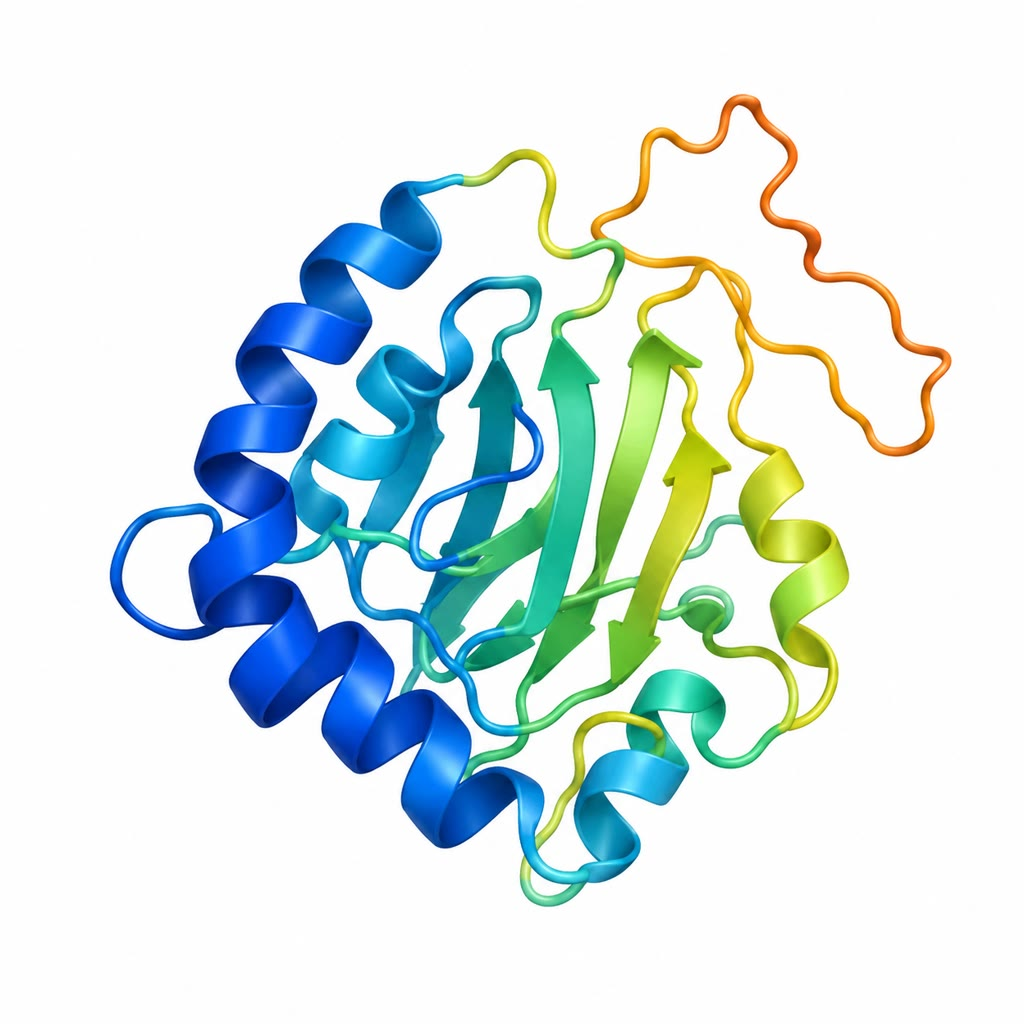
\includegraphics[width=0.36\linewidth]{images/book5/ai/b5-05-alphafold.jpg}\hspace{0.04\linewidth}
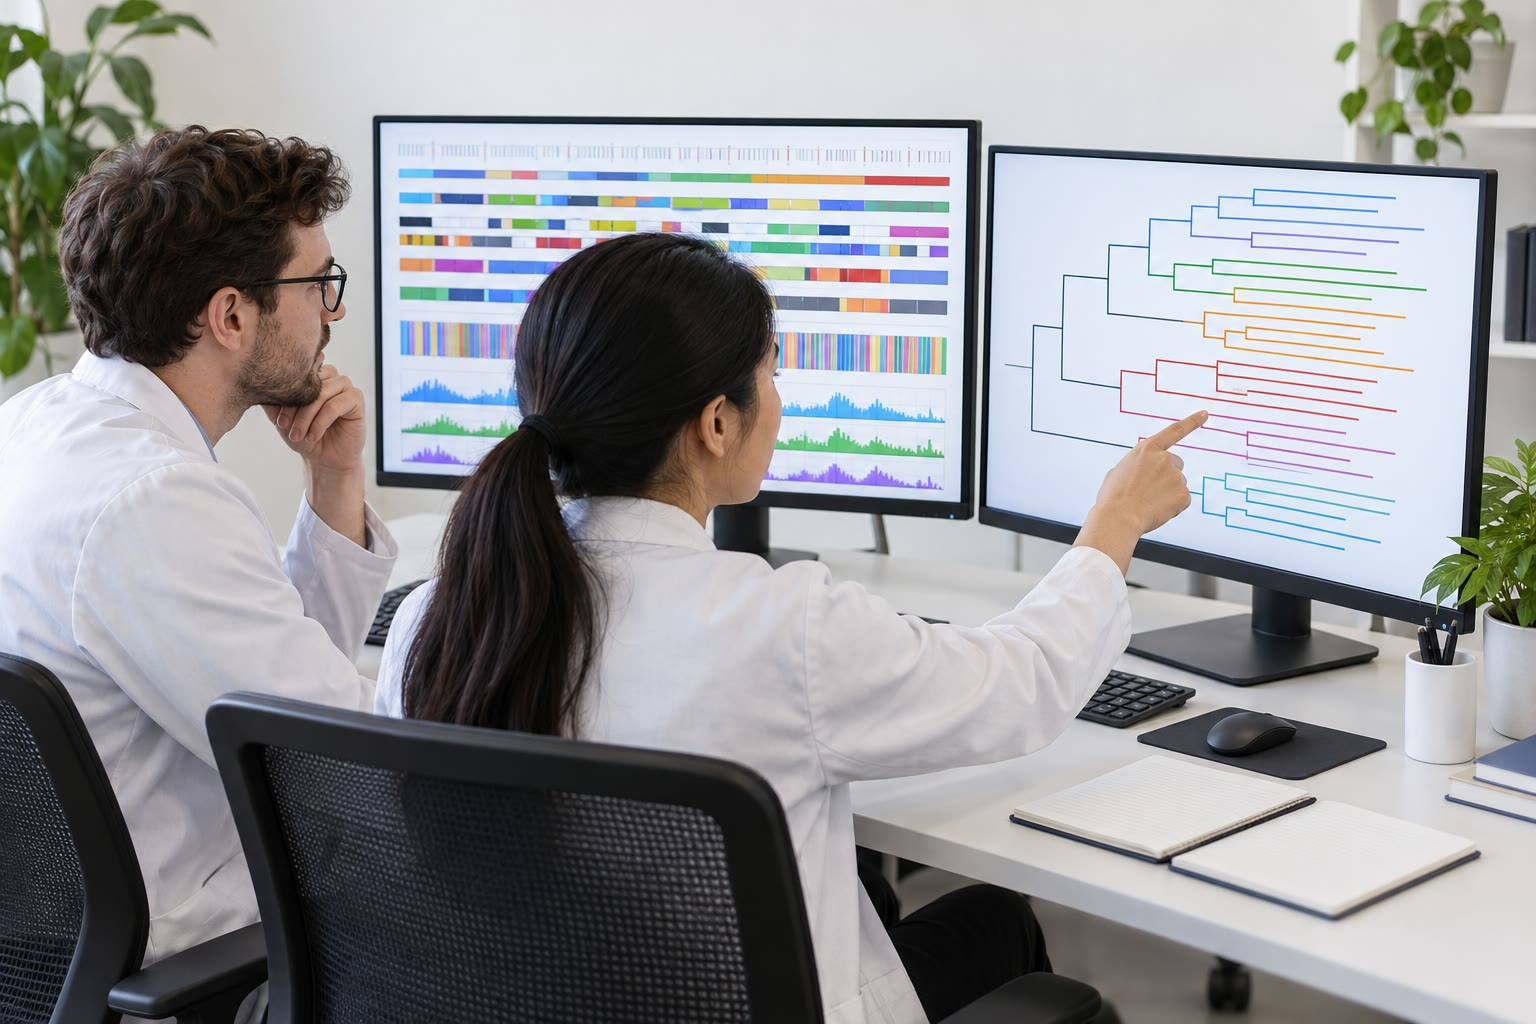
\includegraphics[width=0.54\linewidth]{images/book5/ai/b5-05-bioinformatics-lab.jpg}

{\small À gauche~: une structure de protéine prédite, colorée selon la
confiance du modèle, du fort (bleu) au faible (orange) dans une boucle
désordonnée. À droite~: un bureau de bio-informatique --- des
navigateurs de génomes et des arbres sur les écrans, et pas une
paillasse en vue.}
\end{omfigure}

\begin{remark}[Les limites de l'inférence]\label{rem:b3:bioinformatics:limits}
La plupart des \omterm{def:b3:genomics:assembly}{annotations} fonctionnelles des bases de données n'ont
jamais été testées~; elles ont été transférées depuis un homologue,
lui-même annoté par transfert. Les erreurs se propagent et se
multiplient, et une \omterm{def:b3:genomics:assembly}{annotation} fausse sur une protéine bien connectée
peut contaminer toute une famille. Les remèdes sont ceux d'en haut~:
distinguer l'orthologie de l'homologie, lire l'\omterm{def:b3:bioinformatics:alignment}{alignement}, chercher les
résidus catalytiques, et se souvenir que «~protéine hypothétique~» est
une étiquette honnête que méritent encore un tiers des gènes de la
plupart des génomes.
\end{remark}

\section{Exercices}

\begin{exercise}[$\star$]\label{exo:b3:bioinformatics:1}
Définir \omterm{def:b3:bioinformatics:alignment}{alignement global} et \omterm{def:b3:bioinformatics:alignment}{alignement local}, et donner une situation
biologique qui appelle chacun d'eux.
\end{exercise}

\begin{exercise}[$\star$]\label{exo:b3:bioinformatics:2}
Remplir le tableau de Needleman--Wunsch pour AGC contre AAC avec
correspondance $+1$, mésappariement $-1$, brèche $-1$, et donner
l'\omterm{def:b3:bioinformatics:alignment}{alignement} optimal et son score.
\end{exercise}

\begin{exercise}[$\star$]\label{exo:b3:bioinformatics:3}
Dans BLOSUM62, tryptophane--tryptophane vaut $+11$ et
leucine--leucine $+4$. Expliquer, à partir de la formule de log-cote,
pourquoi l'identité du résidu le plus rare vaut davantage.
\end{exercise}

\begin{exercise}[$\star$]\label{exo:b3:bioinformatics:4}
Qu'est-ce qu'une \omterm{thm:b3:bioinformatics:evalue}{valeur E}~? Une recherche renvoie une correspondance
avec $E = 3$. Que signifie ce nombre, et cette correspondance est-elle
un homologue~?
\end{exercise}

\begin{exercise}[$\star\star$]\label{exo:b3:bioinformatics:5}
Une requête de \num{400} résidus est cherchée dans $2\times 10^{11}$
résidus. Calculer la \omterm{thm:b3:bioinformatics:evalue}{valeur E} des correspondances de \omterm{thm:b3:bioinformatics:evalue}{scores en bits}
$45$, $55$ et $65$. Quel \omterm{thm:b3:bioinformatics:evalue}{score en bits} donne $E = 10^{-3}$~? Comment la
réponse change-t-elle si la requête ne fait que \num{40} résidus~?
\end{exercise}

\begin{exercise}[$\star\star$]\label{exo:b3:bioinformatics:6}
Calculer le \omterm{def:b3:bioinformatics:motif}{contenu en information} d'un \omterm{def:b3:bioinformatics:motif}{motif} dont les quatre positions
ont pour fréquences de bases (A, C, G, T) $(1,0,0,0)$,
$(0.5,0,0.5,0)$, $(0.25,0.25,0.25,0.25)$ et $(0.7,0.1,0.1,0.1)$.
Combien de correspondances fortuites a-t-il dans un génome de
\qty{4.6}{Mb}~?
\end{exercise}

\begin{exercise}[$\star\star$]\label{exo:b3:bioinformatics:7}
Expliquer pourquoi les \omterm{def:b3:bioinformatics:alignment}{pénalités de brèche} affines sont plus réalistes
que les linéaires, et pourquoi une pénalité d'ouverture très forte et
une très faible donnent toutes deux de mauvais \omterm{def:b3:bioinformatics:alignment}{alignements}.
\end{exercise}

\begin{exercise}[$\star\star$]\label{exo:b3:bioinformatics:8}
Une recherche \omterm{def:b3:bioinformatics:blast}{BLAST} d'une protéine humaine contre une base de mouche
donne une meilleure correspondance à $E = 10^{-30}$ couvrant les
résidus 50--180 d'une requête de \num{600} résidus. La protéine de
mouche est-elle l'\omterm{def:b3:genomics:comparative}{orthologue} de la protéine humaine~? Quel test
supplémentaire feriez-vous~?
\end{exercise}

\begin{exercise}[$\star\star$]\label{exo:b3:bioinformatics:9}
Pourquoi les méthodes de \omterm{def:b3:bioinformatics:msa}{profil} détectent-elles des homologues que
l'\omterm{def:b3:bioinformatics:alignment}{alignement} par paires manque~? Donner l'exemple d'un \omterm{def:b3:bioinformatics:motif}{motif} de colonne
qu'un \omterm{def:b3:bioinformatics:msa}{profil} saisit et qu'une séquence unique ne peut pas saisir.
\end{exercise}

\begin{exercise}[$\star\star\star$]\label{exo:b3:bioinformatics:10}
Montrer que, sous un système de score de \omterm{prop:b3:bioinformatics:logodds}{score espéré} positif,
l'\omterm{def:b3:bioinformatics:alignment}{alignement local} de Smith--Waterman de deux longues séquences
aléatoires a un score qui croît linéairement avec leur longueur, et
expliquer pourquoi cela fait échouer la théorie des \omterm{thm:b3:bioinformatics:evalue}{valeurs E}.
Qu'est-ce que cela implique pour l'\omterm{def:b3:bioinformatics:alignment}{alignement} d'ADN avec correspondance
$+1$ et mésappariement $-1$ à \qty{60}{\%} de GC~?
\end{exercise}

\begin{exercise}[$\star\star\star$]\label{exo:b3:bioinformatics:11}
Le tableau de Needleman--Wunsch demande $mn$ cases de mémoire~; pour
deux chromosomes de \qty{100}{Mb} cela fait $10^{16}$. Décrire deux
idées par lesquelles les aligneurs de génomes s'en dispensent (amorces
et chaînage~; bande), et ce que chacune abandonne.
\end{exercise}

\begin{exercise}[$\star\star\star$]\label{exo:b3:bioinformatics:12}
Un HMM de recherche de gènes bactériens a des états pour les trois
positions du codon et pour l'ADN non codant. Expliquer comment le
modèle peut distinguer le codant du non-codant sans aucune information
sur les codons stop (penser à l'usage des codons), et pourquoi la même
approche est bien plus difficile dans un génome humain.
\end{exercise}

\section{Problème~: une séquence des grands fonds}

\begin{problem}[{Problème du week-end --- une protéine inconnue alignée
à la main, cherchée dans les bases de données avec calcul de sa
signification, son motif régulateur pesé en bits et son gène confronté
à la statistique des cadres de lecture ouverts aléatoires, pour finir
sur la valeur E de la meilleure correspondance, les bits qu'exige un
site et la longueur qu'un cadre de lecture doit avoir pour être cru}]
\label{pb:b3:bioinformatics:1}
Données~: une protéine de \num{300} résidus d'un annélide des grands
fonds. Base de protéines~: $1.2\times 10^{11}$ résidus. Génome du ver~:
\qty{1.6}{Gb}, \qty{38}{\%} de GC. Score des \omterm{def:b3:bioinformatics:alignment}{alignements} à la main~:
correspondance $+1$, mésappariement $-1$, brèche $-1$. \omterm{thm:b3:bioinformatics:evalue}{Score en bits} de
la meilleure correspondance \omterm{def:b3:bioinformatics:blast}{BLAST}~: $92$~; de la dixième~: $38$.

\medskip
\noindent\textbf{Partie I --- À la main.}
\begin{enumerate}
  \item Aligner les peptides KQT et KAQT par la récurrence de
        Needleman--Wunsch~: écrire le tableau et donner l'\omterm{def:b3:bioinformatics:alignment}{alignement}
        optimal et son score.
  \item Recommencer avec Smith--Waterman (local) pour GATCAT contre
        ACAT~: trouver le meilleur \omterm{def:b3:bioinformatics:alignment}{alignement local} et son score.
  \item Combien de mises à jour de cases demande un \omterm{def:b3:bioinformatics:alignment}{alignement global}
        de la protéine de \num{300} résidus contre une protéine de
        \num{450} résidus~? Et contre la base entière~?
  \item Si un ordinateur effectue $10^{9}$ mises à jour par seconde,
        combien de temps prend l'\omterm{def:b3:bioinformatics:alignment}{alignement} complet de la base de la
        question 3~? Pourquoi emploie-t-on \omterm{def:b3:bioinformatics:blast}{BLAST} à la place~?
  \item Un score d'identité BLOSUM62 vaut $+4$ pour l'alanine ($p_{A} =
        0.074$) et $+11$ pour le tryptophane ($p_{W} = 0.013$). Avec
        $\lambda = 0.347$ (unités de demi-bit), calculer les fréquences
        cibles $q_{AA}$ et $q_{WW}$, ainsi que le rapport $q/p^{2}$
        pour chacune. Interpréter.
  \item Deux protéines partagent \qty{24}{\%} d'identité sur $250$
        résidus. Dire pourquoi l'identité seule ne peut pas trancher
        l'homologie ici, et ce qui le pourrait.
\end{enumerate}

\medskip
\noindent\textbf{Partie II --- La recherche.}
\begin{enumerate}[resume]
  \item Calculer $mn$ pour la requête contre la base, et
        $\log_{2}(mn)$.
  \item Calculer la \omterm{thm:b3:bioinformatics:evalue}{valeur E} de la meilleure correspondance
        ($S' = 92$) et de la dixième ($S' = 38$).
  \item Quel \omterm{thm:b3:bioinformatics:evalue}{score en bits} correspond à $E = 10^{-3}$ pour cette
        recherche~? Et à $E = 1$~?
  \item La même meilleure correspondance est trouvée alors que la base
        a grossi jusqu'à $1.2\times 10^{12}$ résidus. Sa \omterm{thm:b3:bioinformatics:evalue}{valeur E}~?
  \item La dixième correspondance aligne les résidus 200--260 de la
        requête avec \qty{40}{\%} d'identité sur $60$ résidus. À l'aide
        de la \omterm{thm:b3:bioinformatics:evalue}{valeur E}, dire si c'est une preuve d'homologie, et ce
        qu'une recherche par \omterm{def:b3:bioinformatics:msa}{profil} pourrait y ajouter.
  \item La meilleure correspondance est une kinase humaine, alignée sur
        les résidus 10--290. Sa meilleure correspondance dans le
        protéome du ver est la requête. Qu'établit ce test réciproque,
        et que n'établit-il pas~?
\end{enumerate}

\medskip
\noindent\textbf{Partie III --- Un \omterm{def:b3:bioinformatics:motif}{motif}.}
\begin{enumerate}[resume]
  \item En amont du gène se trouve un site candidat de facteur de
        transcription, de huit positions, de \omterm{def:b3:bioinformatics:motif}{contenus en information}
        $2, 2, 1.6, 2, 0.8, 1.2, 0.4, 0.3$ bits. Total $R$~?
  \item Combien de correspondances fortuites ce \omterm{def:b3:bioinformatics:motif}{motif} a-t-il dans le
        génome de \qty{1.6}{Gb} (les deux brins, $3.2\times 10^{9}$
        positions)~?
  \item Le facteur règle environ $200$ gènes. Combien de bits faudrait-il
        à un \omterm{def:b3:bioinformatics:motif}{motif} pour spécifier seul $200$ sites dans ce génome~?
  \item Quelle part du manque un second \omterm{def:b3:bioinformatics:motif}{motif} voisin de $8$ bits
        pourrait-il fournir, si les deux doivent se rencontrer à un
        espacement fixé~?
  \item Une position de fréquences $(0.5, 0.5, 0, 0)$ pour (A, C, G,
        T)~: calculer son entropie et son \omterm{def:b3:bioinformatics:motif}{contenu en information}.
  \item Expliquer, par l'argument informationnel, pourquoi les facteurs
        de transcription bactériens ont d'ordinaire des sites plus
        longs et plus conservés que les eucaryotes.
\end{enumerate}

\medskip
\noindent\textbf{Partie IV --- Le gène lui-même.}
\begin{enumerate}[resume]
  \item Dans un ADN aléatoire de composition en bases uniforme, quelle
        est la probabilité qu'un codon soit un stop~? Quel est le
        nombre espéré de codons avant l'apparition d'un stop (loi
        géométrique)~?
  \item Le génome du ver a \qty{38}{\%} de GC. Recalculer la
        probabilité qu'un codon aléatoire soit un stop (TAA, TAG, TGA)
        avec les fréquences de bases réelles, et la longueur espérée du
        cadre de lecture. Dans quel sens une faible teneur en GC
        pousse-t-elle la recherche de gènes~?
  \item Quelle est la probabilité qu'un cadre de lecture ouvert
        aléatoire compte au moins $100$ codons~? Au moins $300$~?
  \item Dans le génome de \qty{1.6}{Gb}, six cadres sur deux brins
        donnent environ $3.2\times 10^{9}$ départs de codons. Combien
        de cadres de lecture ouverts aléatoires d'au moins $100$ codons
        attend-on~? Et d'au moins $300$~?
  \item Expliquer pourquoi «~cadre de lecture ouvert de plus de $100$
        codons~» est un chercheur de gènes utilisable chez une bactérie
        mais non dans ce génome, et ce qu'un chercheur de gènes
        eucaryote emploie à la place.
  \item Le gène du ver a six exons de \qty{150}{bp} en moyenne.
        Expliquer comment des lectures de séquençage d'ARN résolvent la
        structure en exons que la séquence génomique seule laisse
        ambiguë.
  \item Résumer~: la \omterm{thm:b3:bioinformatics:evalue}{valeur E} de la meilleure correspondance
        (question~8), les bits nécessaires pour spécifier $200$ sites
        (question~15) et le nombre espéré de cadres de lecture
        aléatoires de $300$ codons dans le génome (question~22).
\end{enumerate}
\end{problem}
